\documentclass{prova}

\usepackage{amssymb}
\usepackage{gensymb}

\renewcommand{\sin}{\mbox{sen}}
\newcommand{\ra}{\rightarrow}
\newcommand{\lra}{\leftrightarrow}
\newcommand{\Ra}{\Rightarrow}
\newcommand{\LRa}{\Leftrightarrow}
\renewcommand{\lnot}{\sim}
\newcommand{\larg}{\vdash}
\newcommand{\ds}{\displaystyle}
\newcommand{\sen}{\mathop\mathrm{sen}\nolimits}
\newcommand{\tg}{\mathop\mathrm{tg}\nolimits}
\newcommand{\cotg}{\mathop\mathrm{cotg}\nolimits}
\newcommand{\cossec}{\mathop\mathrm{cossec}\nolimits}

\professor{Prof. Adriano Barbosa}
\disciplina{Introdução ao Cálculo}
\avaliacao{P1}
\curso{Matem\'atica}
\data{20/11/2020}

\begin{document}
    \cabecalho{5}  % o numero 5 indica a qnt de quadros na tabela de nota
    
    \textbf{Todas as respostas devem ser justificadas.}
    \begin{questionario}
        \q{}
            \begin{questionario}
                \qq{Determine a fração irredutível igual ao número
                    $3,47373737373...$.}
                \qq{O número $0,102030405060708090100110120...$ pode ser
                    escrito como uma fração?}
            \end{questionario}
        \q{Determine os algarismos que faltam em cada fração:}
            \begin{questionario}
                \qq{$\displaystyle\frac{48}{6\,\_\!\_}=\frac{4}{\_\!\_}$}
                \qq{$\displaystyle\frac{\_\!\_\,\_\!\_\,5}{25\,\_\!\_}=\frac{53}{17}$}
            \end{questionario}
        \q{Represente geometricamente os invervalos abaixo na reta real:}
            \begin{figure}[h]
                \centering
                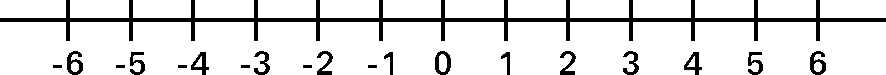
\includegraphics[width=0.5\textwidth]{fig1.pdf}
            \end{figure}
            \begin{questionario}
                \qq{$\ds \left[-\frac{5}{2},-1\right]$}
                \qq{$\ds \left(0,\pi\right]$}
                \qq{$\ds \left(-2,4\right)$}
                \qq{$\ds \left[-\frac{5}{2},-1\right]\cup\left(0,\pi\right]$}
                \qq{$\ds \left[-\frac{5}{2},-1\right]\cap\left(-2,4\right)$}
            \end{questionario}
        \q{Mostre que a função $f:\mathbb{R}-\{-1\}\rightarrow\mathbb{R}-\{1\}$,
           $\ds f(x)=\frac{x}{1+x}$ é uma bijeção e encontre a expressão da sua inversa.}
        \q{Dadas as funções $f$ e $g$ cujas regras são
           $f(x)=\sqrt{x}$ e $\ds g(x)=\frac{1}{x^2-4}$, determine o maior subconjunto de
           $\mathbb{R}$ onde a composta $g(f(x))$ está bem definida e determine a regra
           da composta.}
    \end{questionario}
\end{document}
